%\section{Ограниченост на популациите}

\begin{frame}[t]{Ограниченост на популациите}

\begin{block}{Популацията при динамика на Бевъртън-Холт е ограничена}
Нека $x(n+1)=x(n)\frac{a}{b x(n) + 1}, a > 0, b > 0,x(0) \geq 0$. \\
\begin{enumerate}[I]

\item $a \in \left(0, 1 \right]$: $x(n+1) \leq a x(n) \leq x(n)$ и $x(n) \xrightarrow[n \to \infty]{\text{монотонно}} 0$


\item $a > 1$: $\frac{x(n+1)}{x(n)}=\frac{a}{b x(n) + 1}, \frac{a}{b x(n) + 1} = 1 \iff x(n) = \frac{a-1}{b}$
\begin{enumerate}

\item $x(0) \in \left(0, \frac{a-1}{b} \right)$: Тогава $\frac{a}{b x(n) + 1} > 1$ и $x(n) \xrightarrow[n \to \infty]{\text{монотонно}} \frac{a-1}{b}$

\item $x(0) > \frac{a-1}{b}$: Тогава $\frac{a}{b x(n) + 1} < 1$ и $x(n) \xrightarrow[n \to \infty]{\text{монотонно}} \frac{a-1}{b}$

\end{enumerate}


\end{enumerate}


Следователно популацията е ограничена от $\max \{x(0), \frac{a-1}{b}\}$.
%\[\max \{x(0), \frac{a-1}{b}\}\]


%Сл.1 : $a \in \left[0, 1 \right]$ \\
%\quad $x(n+1)<x(n)\frac{a}{1}=a x(n) \leq x(n)$, тоест:
%$\forall{n} \;  x \left(n \right) \leq x(0)$.\\
%Сл.2 : $a > 1$ \\
%\quad $x(n+1)<x(n)\frac{a}{1}=a x(n) < x(n)$, тоест:
%$\forall{n} \;  x \left(n \right) \leq x(0)$.

\end{block}

\end{frame}


\begin{frame}[t]{Ограниченост на популациите}


\begin{center}


\begin{figure}
\begin{tabular}{c c}
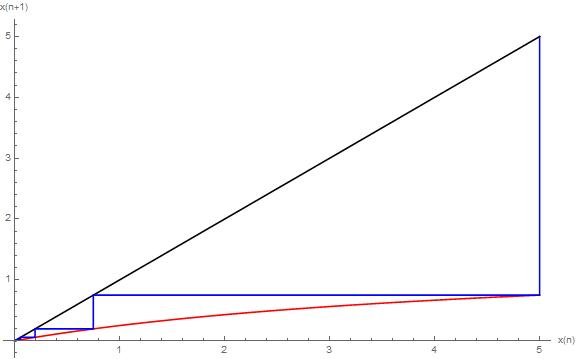
\includegraphics[width=4.5cm,height=4cm]{climbing1} &
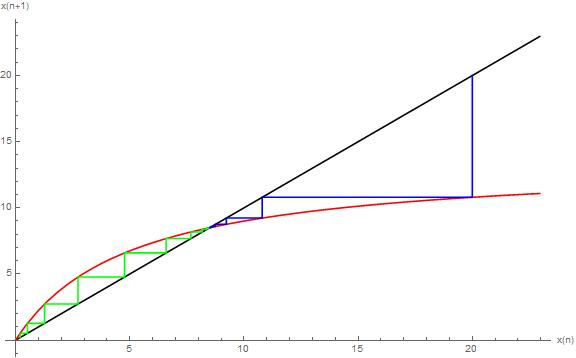
\includegraphics[width=6cm,height=4cm]{climbing2} \\
{$0 < a \leq 1$} & {$a > 1$} \\
\end{tabular}
\end{figure}

\end{center}

\end{frame}


\begin{frame}[t]{Ограниченост на популациите}

\begin{block}{При Бевъртън-Холт мажориращи начални условия водят до мажориращи решения}
Нека $x(n+1)=x(n)\frac{a}{b x(n) + 1}, a > 0, b > 0,x(0) \geq 0$. \\
Параметризирайки по началното условие $x(0) = x_{0}$: \\
$x(n+1,x_{0})= x(n,x_{0})\frac{a}{b x(n,x_{0}) + 1}, a > 0, b > 0,x(0, x_{0}) = x_{0} \geq 0$. \\
Нека са дадени начални условия $\theta_{1}, \theta_{2}, \theta_{1} \geq \theta_{2}$. Тогава е в сила, че $\forall{n} \; x(n,\theta_{1}) \geq x(n,\theta_{2})$. Доказваме чрез индукция по $n$:
\begin{itemize}
\item $x(0, \theta_{1}) = \theta_{1} \geq \theta_{2} = x(0, \theta_{2})$
\item $x(n+1, \theta_{1}) - x(n+1, \theta_{2}) =\frac{a x(n,\theta_{1})}{b x(n,\theta_{1}) + 1} - \frac{a x(n,\theta_{2})}{b x(n,\theta_{2}) + 1} = \frac{a (x(n,\theta_{1}) - x(n,\theta_{2}))}{b^{2} x(n,\theta_{1}) x(n,\theta_{2}) + b(x(n,\theta_{1}) + x(n,\theta_{2})) + 1} \geq 0$
\end{itemize}

\end{block}

\end{frame}



\begin{frame}[t]{Ограниченост на популациите}

Достатъчно за четната подредица е да покажем, че $\forall{n} \; x_{1} \left(2n \right) + x_{2} \left(2n \right) < M$ за някое $M$, тъй като $x_{i} \left(2n \right) \geq 0 \implies x_{i} \left(2n \right) \leq x_{1} \left(2n \right) + x_{2} \left(2n \right) < M, \enspace i=1,2$. \\
Допълнително, ограничеността на четната подредица влече ограничеността на нечетната:
\[x_{i} \left(2n+1 \right) = x_{i} \left(2n \right) \frac{a_{i}}{1 + b_{i} x_{i} \left(2n \right)} \leq x_{i} \left(2n \right) a_{i} < a_{i} M = M_{i}', i=1, 2\]
Тогава като дефинираме
$M' = \max \{M_{1}',M_{2}',M\}$, то $\forall{n} \; x_{i} \left(n  \right) < M'$. \\

\end{frame}

\begin{comment}

\begin{frame}[t]{Ограниченост на популациите}

%Да допуснем, че $\exists{i \in \{1,2\}} \, \forall{M} \, \exists{n'} \, \forall{n \geq n'} \;  y_{i} \left(n \right) \geq M$. \\

%Случай 1: $\{y_{1}(n)\}_{n=0}^{\infty}, \{y_{2}(n)\}_{n=0}^{\infty}$ са неограничени. \\
%\quad Тогава, стига $y_{1}(n), y_{2}(n)$ да са достатъчно големи: $y_{1}(n+1)+y_{2}(n+1)=y_{1}(n) \frac{\alpha_{1} a_{1}}{(a_{1} \beta_{1} + b_{1}) y_{1}(n) + 1} + y_{2}(n) \frac{\alpha_{2} a_{2}}{(a_{2} \beta_{2} + b_{2}) y_{2}(n) + 1} \leq$ $\leq y_{1}(n)+y_{2}(n)$ \\
%Случай 2: Само $\{y_{i}(n)\}_{n=0}^{\infty}$ е неограничена.


Знаем, че: $y_{1}(n+1)+y_{2}(n+1)=y_{1}(n) \frac{\alpha_{1} a_{1}}{(a_{1} \beta_{1} + b_{1}) y_{1}(n) + 1} + y_{2}(n) \frac{\alpha_{2} a_{2}}{(a_{2} \beta_{2} + b_{2}) y_{2}(n) + 1}$ \\
Но сумата може да се замени от следната, оставайки същата: \\
$\xi_{1}(n+1)+\xi_{2}(n+1)=\xi_{1}(n) \frac{\alpha_{1} a_{1}}{(a_{1} \beta_{1} + b_{1}) \xi_{1}(n) + 1} + \xi_{2}(n) \frac{\alpha_{2} a_{2}}{(a_{2} \beta_{2} + b_{2}) \xi_{2}(n) + 1}$
Но може да дефинираме динамика за $\xi$:
\[\xi_{1}(n+1)=\xi_{1}(n) \frac{\alpha_{1} a_{1}}{(a_{1} \beta_{1} + b_{1}) \xi_{1}(n) + 1}\]
\[\xi_{2}(n+1)=\xi_{2}(n) \frac{\alpha_{2} a_{2}}{(a_{2} \beta_{2} + b_{2}) \xi_{2}(n) + 1}\]
Тук $\xi_{i}(0)=y_{i}(0),\enspace i=1,2$ \\
Сега свеждаме проблема до ограничеността на популация при стандартната динамика на Бевъртън-Холт.

\end{frame}

\end{comment}


\begin{frame}[t]{Ограниченост на популациите}

Нека $A=\max \{\alpha_{1} a_{1},\alpha_{2} a{2}\}, B=\min \{a_{1} \beta_{1} + b_{1},a_{2} \beta_{2} + b_{2}\}$. Следва:
$y_{i}(n+1) \leq y_{1}(n) \frac{A}{B y_{1}(n) + 1} + y_{2}(n) \frac{A}{B y_{2}(n) + 1}$. Тогава нека дефинираме динамиката за $\boldsymbol{\xi}$:
\[\xi_{1}(n+1) = \xi_{1}(n) \frac{A}{B \xi_{1}(n) + 1} + \xi_{2}(n) \frac{A}{B \xi_{2}(n) + 1}, \enspace \xi_{1}(0)=y_{1}(0)\]
\[\xi_{2}(n+1) = \xi_{1}(n) \frac{A}{B \xi_{1}(n) + 1} + \xi_{2}(n) \frac{A}{B \xi_{2}(n) + 1}, \enspace \xi_{2}(0)=y_{2}(0)\]
Така $\forall{n} \; \xi_{i}(n) \geq y_{i}(n)$. Но $\forall{n} \; \xi_{1}(n+1)=\xi_{2}(n+1)$. Остава да проверим ограничеността на следната динамика:
\[\hat{\xi}(n+1) = \hat{\xi}(n) \frac{2 A}{B \hat{\xi}(n) + 1}, \hat{\xi}(0)=\xi_{1}(0) \frac{A}{B \xi_{1}(0) + 1} + \xi_{2}(0) \frac{A}{B \xi_{2}(0) + 1}\]
Но това е динамика на Бевъртън-Холт, която е ограничена по доказаното по-горе свойство.
%Тя е ограничена, по показаното по-горе свойство, откъдето $\xi_{i}$ са ограничени, т.е. $y_{i}$ са ограничени и съответно $x_{i}$

\end{frame}
